\documentclass{standalone}
% This file was created with tikzplotlib v0.9.15.

\usepackage{siunitx}
\usepackage{pgfplots}
% and optionally (as of Pgfplots 1.3):
\pgfplotsset{compat=newest}
\pgfplotsset{plot coordinates/math parser=false}
\newlength\figureheight
\newlength\figurewidth

\newcommand{\Set}[1]{\mathcal{#1}}
\newcommand{\Vector}[1]{\bm{\MakeLowercase{#1}}}
\newcommand{\Operator}[1]{\bm{\MakeUppercase{#1}}}
%%%%%%%%%%
\DeclareMathAlphabet{\mathsfbr}{OT1}{cmss}{m}{n}%for math sans serif (cmss)
\SetMathAlphabet{\mathsfbr}{bold}{OT1}{cmss}{bx}{n}%for math sans serif (cmss)
\DeclareRobustCommand{\msf}[1]{%
  \ifcat\noexpand#1\relax\msfgreek{#1}\else\mathsfbr{#1}\fi%for math sans serif (cmss)
}
\DeclareFontEncoding{LGR}{}{} % or load \usepackage{textgreek}
\DeclareSymbolFont{sfgreek}{LGR}{cmss}{m}{n}
\SetSymbolFont{sfgreek}{bold}{LGR}{cmss}{bx}{n}
\DeclareMathSymbol{\sXi}{\mathalpha}{sfgreek}{`X}
\DeclareMathSymbol{\sUpsilon}{\mathalpha}{sfgreek}{`U}

\begin{document}

% This file was created with tikzplotlib v0.9.15.
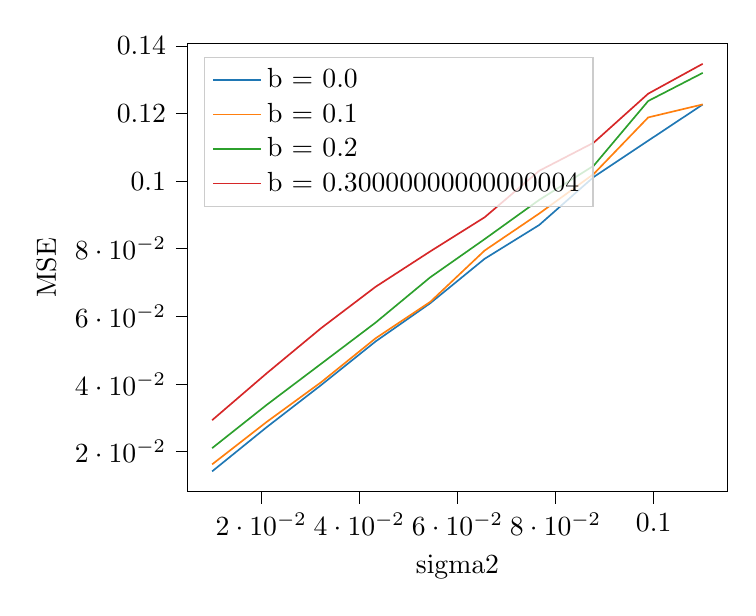
\begin{tikzpicture}

\definecolor{color0}{rgb}{0.12156862745098,0.466666666666667,0.705882352941177}
\definecolor{color1}{rgb}{1,0.498039215686275,0.0549019607843137}
\definecolor{color2}{rgb}{0.172549019607843,0.627450980392157,0.172549019607843}
\definecolor{color3}{rgb}{0.83921568627451,0.152941176470588,0.156862745098039}

\begin{axis}[
legend cell align={left},
legend style={
  fill opacity=0.8,
  draw opacity=1,
  text opacity=1,
  at={(0.03,0.97)},
  anchor=north west,
  draw=white!80!black
},
tick align=outside,
tick pos=left,
x grid style={white!69.0196078431373!black},
xlabel={sigma2},
xmin=0.005, xmax=0.115,
xtick style={color=black},
y grid style={white!69.0196078431373!black},
ylabel={MSE},
ymin=0.0081403, ymax=0.1407057,
ytick style={color=black}
]
\addplot [semithick, color0]
table {%
0.01 0.014166
0.0211111111111111 0.027222
0.0322222222222222 0.039686
0.0433333333333333 0.0526
0.0544444444444444 0.063872
0.0655555555555556 0.077032
0.0766666666666667 0.08701
0.0877777777777778 0.101222
0.0988888888888889 0.11195
0.11 0.122648
};
\addlegendentry{b = 0.0}
\addplot [semithick, color1]
table {%
0.01 0.01624
0.0211111111111111 0.02878
0.0322222222222222 0.040528
0.0433333333333333 0.053526
0.0544444444444444 0.064258
0.0655555555555556 0.079478
0.0766666666666667 0.090398
0.0877777777777778 0.102102
0.0988888888888889 0.118824
0.11 0.12267
};
\addlegendentry{b = 0.1}
\addplot [semithick, color2]
table {%
0.01 0.021032
0.0211111111111111 0.03382
0.0322222222222222 0.045982
0.0433333333333333 0.058172
0.0544444444444444 0.071532
0.0655555555555556 0.082844
0.0766666666666667 0.094432
0.0877777777777778 0.104546
0.0988888888888889 0.123686
0.11 0.13199
};
\addlegendentry{b = 0.2}
\addplot [semithick, color3]
table {%
0.01 0.029302
0.0211111111111111 0.043156
0.0322222222222222 0.056522
0.0433333333333333 0.068756
0.0544444444444444 0.079198
0.0655555555555556 0.089306
0.0766666666666667 0.10304
0.0877777777777778 0.111366
0.0988888888888889 0.125846
0.11 0.13468
};
\addlegendentry{b = 0.30000000000000004}
\end{axis}

\end{tikzpicture}

\end{document}